\begin{frame}{本日の例題}
 
    \begin{columns}[t]
    \begin{column}{0.65\textwidth}
        \\
        <参考文献\cite{wanted} より例題を拝借> \\
        右\figurename \ref{fig:example-probrem}に示すような圧力容器に内圧10MPaが \\
        かかっている。
        材料はSB450で、ヤング率は205GPa、降伏応力は250MPaである。 \\
        本構造は薄肉構造と近似できるとする。
      \begin{itemize}
          \item{円筒部のA点と半球部のB点の応力状態を求めよ}
          \item{A点とB点ミーゼス相当応力を求め、幸福応力に達する臨界圧力を求めよ}
      \end{itemize}
    \end{column}
    \begin{column}{0.35\textwidth}
      \begin{figure}[htbp]
        \begin{center}
          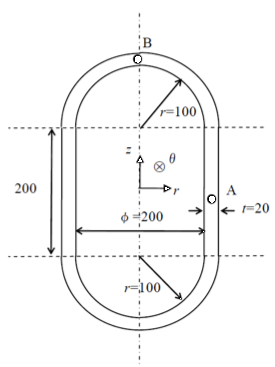
\includegraphics[keepaspectratio,scale=2.2]{work/images/example-probrem.png}
            \caption{本日の例題(圧力容器)} \label{fig:example-probrem}
        \end{center}
      \end{figure}
    \end{column}
  \end{columns}

% 図の挿入
%\begin{figure}[htbp]
%\begin{center}
%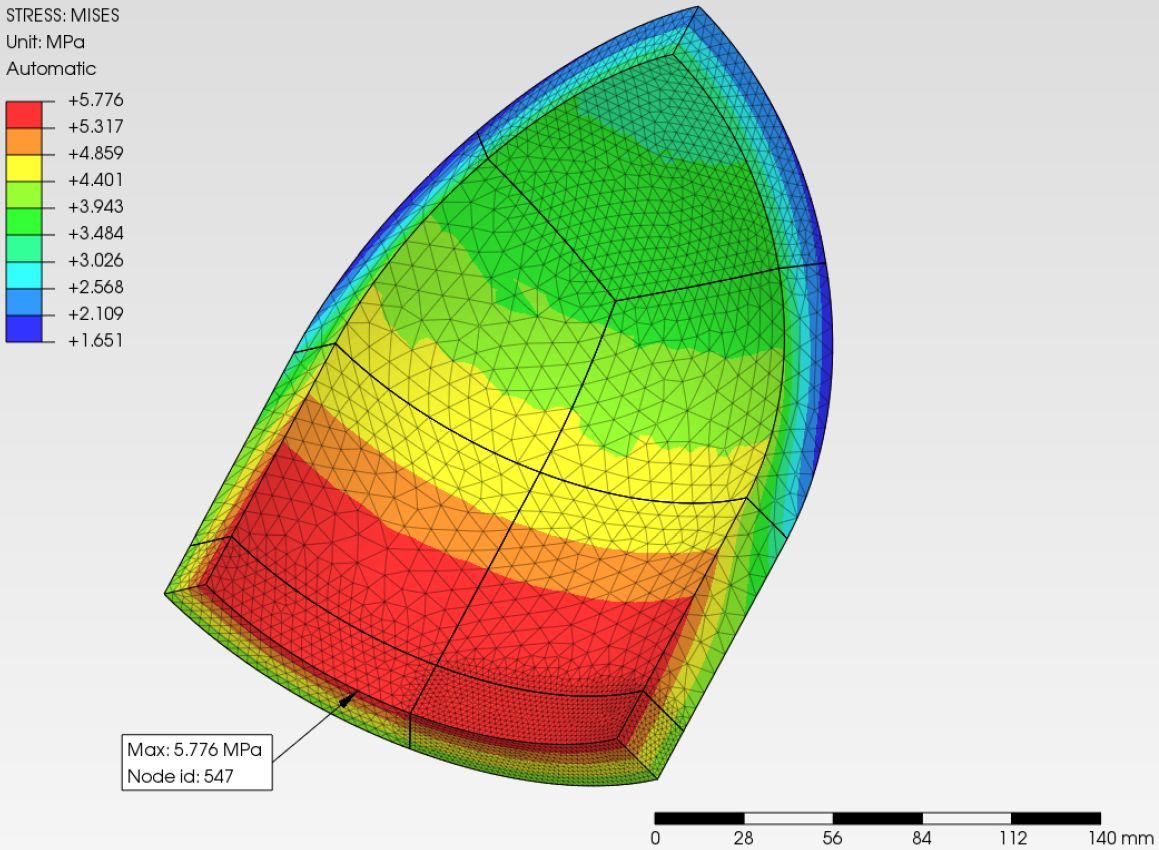
\includegraphics[keepaspectratio,scale=1.0]{work/images/fig01.jpg}
%\caption{4面体メッシュ切り(成功例)}
%\end{center}
%\end{figure}
 
\end{frame}
